\chapter{Preparation} % Typically a mix of background info and initial steps of actual implementation
% Written as if none of the project has actually happened yet? Or written as a reflection of thoughts at the time i.e. I decided that this would be the best choice

% TODO: Figure out best way to order sections

Before implementing my compiler, I researched the structure of WebAssembly programs and the intermediate representations used by the OCaml compiler, as well as possible optimisations to implement. I also considered which best practices to use to ensure that each stage of the project was manageable. % and to identify difficulties early on.

\section{Starting point}
Starting the project, my experience with OCaml was limited to the IB Compiler Construction course and studying the OCaml compiler, looking at the data structures used, and the ASTs generated for some short programs. I decided to build my project on the front-end of the OCaml compiler, after type checking has been performed, since there would be no benefit in reproducing this code. This was chosen rather than the next lower representation in the OCaml compiler, the Lambda language, as it introduces unnecessary structure and operations that would not be needed for the subset of OCaml I aimed to support. 

% Don't just repeat the introduction
I had read parts of the WebAssembly specification to understand the instructions available, and compiled a short C program to WebAssembly to check that I was able to run some of the tools involved.
Many languages can now be compiled to WebAssembly, although lots of tools are still works in progress \cite{langauges-to-wasm}. I chose to compare my compiler against compiling C to WebAssembly, since this appears to be the most matured platform in terms of supporting compilation to WebAssembly \cite{clang-llvm}. I also decided to compare against Grain, as this is a functional language similar to OCaml, and its official compiler emits WebAssembly \cite{grain}. I had not heard of Grain before starting to prepare for the project, so learnt the language from its documentation pages while setting up the tools at the start of my project. Lastly, I considered the performance of the Js\_of\_ocaml tool, which instead produces JavaScript from OCaml code, as this is the most well-known way to run OCaml programs on the web \cite{jsofocaml}.

% NO NEED TO REPEAT ABOUT EXISTING WORK, ALREADY MENTIONED IN INTRODUCTION
%The only example I could find of a compiler from OCaml to WebAssembly was another Part II project from 2020, which worked from the parsed AST produced by the OCaml compiler. By instead working from the typed AST of the compiler, I was able to include a greater subset of OCaml.

% Mention backups

\section{Research undertaken}
For implementing my compiler, I first looked at the approach taken with the OCaml compiler's Lambda intermediate language, and the structure of the Grain compiler. Looking at how translation is done in the OCaml compiler helped to verify that I understood the semantics of the layer I was translating from, and identify the best way to handle specific elements, such as the primitive operations OCaml provides. Grain uses a very different intermediate representation, where operations are linearised so that the arguments to operations are always constants or variables, rather than nested expressions. 
I decided that my intermediate representation should have a linearised structure similar to Grain, since this makes the evaluation order explicit and simplifies implementing optimisation passes. %analysis and optimisation passes on the representation.

%Comparing the two representations helped me to decide on my own intermediate representation for the subset of OCaml I was supporting.

%Grain is a much newer language and is still quickly growing. It supports a subset of OCaml's features but with its own syntax. As it is a much simpler langauge, this was easier to study for working out how to structure translation as a whole, in particular the collections of utility functions I might need for working with my intermediate representation. 

\subsection{Optimisations}
For selecting optimisations to implement, I looked at both the Part IB Compiler Construction \cite{IB-compilers} and Part II Optimising Compilers \cite{optimising-compilers} courses for explanations of a range of optimisations. %Additionally, the Grain compiler implements several optimisation passes, which were helpful to study. 
I also inspected the intermediate code and WebAssembly produced for sample programs, highlighting inefficiencies in translation and identifying where certain optimisations would be beneficial.
%It also became apparent that certain optimisations would be beneficial, after inspecting the intermediate code and WebAssembly produced for sample programs that I wrote, highlighting inefficiencies in the translation stages of the compiler.

The optimisations I chose to implement were:
\begin{itemize}
\item \textbf{Tail-call optimisation}: Rewriting tail-recursive functions to use a \verb|while| loop, rather than making recursive calls, avoids activation frames building up on the call stack, resulting in an error if the available stack space is exceeded.

\item \textbf{Function inlining}: Where the function being called can be identified, a function application can be replaced by substituting it with the body of the function. This can enable further optimisations, possibly at the cost of increasing code size.

\item \textbf{Uncurrying}: Where a function is always applied with several curried arguments, these can be passed as a tuple rather than constructing a closure for each argument in turn, as described by Bloss, Hudak and Young \cite{uncurry}. 

\item \textbf{Constant/Copy propagation}: When a constant or another variable is bound to a variable that will not be overwritten, subsequent uses of that variable can be replaced with its known value, propagating values through the program to identify further optimisations.% This can result in the binding being unused if all uses of the variable are replaced, and propagates values through the program to identify further optimisations.

\item \textbf{Dead-code elimination}: Where a variable is unused (possible due to the previous optimisation) and the value bound to it does not contain side-effects, that binding can be safely removed to reduce code size and execution time.

\item \textbf{Constant folding}: Constant expressions can be evaluated at compile time, such as \verb|1+2|. Branches with constant conditions can also simplified, such as  replacing \verb|if false then e else e'| with \verb|e'|.
%Constant expressions in the program, such as \verb|1+2|, can be evaluated at compile time. Branching statements with constant conditions, such as \verb|if false then e else e'|, can also be replaced with the branch that is guaranteed to execute.

\end{itemize}

The first three optimisations perform relatively complex transformations, requiring analysis to identify where they are both safe and beneficial to perform. The last three optimisations then eliminate redundancy, where some analysis is still necessary to correctly handle expressions with side-effects. This redundancy primarily occurs due to inefficiencies in translation to the intermediate representation, and because of the other optimisations.

% For example, inlining a function means that the values bound to each parameter are now known in the function body, so it may be possible to propagate additional constants etc.

\subsection{Pattern matching}

The Grain and OCaml compilers differ in the techniques used for pattern-matching.  The OCaml compiler implements a backtracking algorithm, which aims to minimise the size of the pattern-matching code produced, whereas the Grain compiler implements a decision-tree algorithm, which ensures that each pattern is examined at most once, minimising execution time. Each implementation references papers on the technique it uses \cite{ocamlpatternmatch, decisiontrees}, which were useful in choosing the approach to take and in understanding how to implement pattern-matching for my intermediate representation.
%
I decided to implement a backtracking pattern-matching compiler.  When optimised, each approach typically has similar performance \cite{decisiontrees}, however backtracking compilers appear to be the more common approach, and guarantee linear code size.


\subsection{WebAssembly}
The majority of my preparation before the start of the project was familiarising myself with the structure of WebAssembly.
This was done by reading the WebAssembly specification \cite{wasm}, as well as some useful articles on how the different components of a WebAssembly module interact in practice \cite{wasm-article}.

WebAssembly is a strongly typed stack-based language. %, where each module additionally has a linear memory, a heap that can be grown in multiples of 64KiB pages and accessed by 32-bit pointers. 
As shown by the example in the introduction (section 1.1), WebAssembly supports nested blocks of instructions, in the form of \verb|Block|, \verb|If| and \verb|Loop| constructs. 

WebAssembly's control flow is very restrictive, only allowing branches out of enclosing blocks rather than arbitrary jumps. A \verb|Br i| or \verb|Br_if i| instruction (conditionally) branches out of the \verb|i|$^{\text{th}}$ enclosing block, jumping to the end of a \verb|Block| or \verb|If| block and to the start of a \verb|Loop| block, allowing loops in the control flow.
%For \verb|Block| and \verb|If| blocks, this branches to the end of the nested instructions. For a \verb|Loop| block, this instead branches to just before the nested instructions, allowing loops in the control flow. % Additionally, a branch to the outermost level of a function acts as a return statement.  -- never actually made use of
%As well as \verb|Br i|, WebAssembly has a conditional \verb|Br_if i| instruction, and branch tables that are indexed by an argument on the stack. 
Exceptions were left out of the subset of OCaml to support, since these restrictions in WebAssembly control flow significantly complicate their implementation, to the extent that exception handling is also disabled by default when compiling C++ to WebAssembly using Clang \cite{wasm-exceptions}.

%WebAssembly is strongly typed, and has four primitive types for 32 and 64-bit integers and floats. Blocks therefore have types, and instructions within a block are unable to access values put on the stack before the start of the block, except for however many .

A WebAssembly module is initialised with a linear memory of a specified number of 64KiB pages, and the size of memory can be queried and expanded during execution.
The memory layout of a native-code program typically has the heap starting at a low address, growing upwards, and the stack starting at a high address and growing down. However, as the stack is managed implicitly in WebAssembly, the linear memory contains just the heap so looks more like figure \ref{fig:wasm-heap}:

% The stack is managed implicitly, so cannot be inspected directly. Whereas a C program compiled to an instruction set such as x86 has the heap start at a low address and grow upwards, with the stack starting at a high address and growing down, WebAssembly memory contains just the first of these components, so memory has the layout shown below:

\begin{figure}[H]
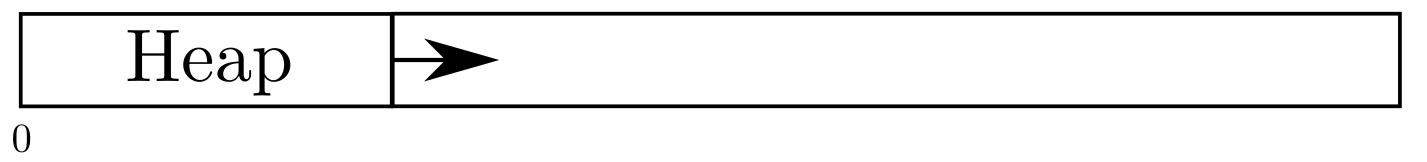
\includegraphics[scale=0.5]{regular_heap}
\caption{Typical WebAssembly memory layout}
\label{fig:wasm-heap}
\end{figure}


\subsection{Garbage collection}
OCaml is a garbage-collected language, so memory is managed automatically. However, memory is managed manually in WebAssembly, so a garbage collector must be implemented in the runtime system to manage objects allocated by compiled OCaml programs.

The two broad categories of garbage collectors are reference-counting and tracing collectors. Reference-counting collectors keep a counter on each object for the number of pointers to that object that exist, freeing the object when the counter falls to zero. This has a high overhead, since a counter needs to be updated whenever a pointer is created or modified, and cyclic structures are never collected. Tracing collectors instead periodically scan a set of root objects that can be accessed directly, and use these to discover all objects indirectly reachable from them. Any object not marked as reachable is then safe to free. 

WebAssembly's implicit stack cannot be accessed directly, which complicates garbage collection as the values on the stack are part of the root set and need to be scanned during garbage collection. Therefore, garbage collection was left as an extension due to the challenges surrounding it. One solution is to implement a shadow stack in the linear memory, which stores a copy of each local variable saved on the implicit stack, allowing these to be traversed during garbage collection. Shadow stacks are more common in the context of security, where a function's return address is copied elsewhere in memory and compared when the function returns, detecting attempts to overwrite the return address on the stack \cite{shadow-stack}. % For performing garbage collection, a copy of each local variable is saved to the shadow stack, and garbage collection scans this region of memory to identify reachable pointers. 

The shadow stack must extend upwards from the start of the linear memory, since WebAssembly memory grows over time so the top of the address space is not initially valid. Therefore, the top of the stack is limited by the starting position of the heap, and the layout of memory is as shown in figure \ref{fig:wasm-shadow}. %This is not a significant issue, as it was already possible to generate a stack-overflow error, by exhausting the available space in the underlying platform's implementation of the implicit stack. Using a shadow stack, the layout of linear memory is therefore as shown below:


%The WebAssembly memory now starts with the shadow stack, which can extend up to a fixed limit, after which the heap begins. This creates the possibility of a stack overflow error occurring, but such errors were already possible from the platform's implementation of the implicit stack, before garbage collection was added. It is not possible to have the stack and heap grow from opposite ends of memory, as typically happens in C, since the WebAssembly memory is initially small, so large blocks of memory would have to be copied to new locations when the memory grows. With garbage collection, memory therefore has the layout shown below:


% Mention the difficulties of garbage collection and the use of shadow stack
%The stack is managed implicitly, which is an issue for garbage collection since it means there is no way to scan the stack to discover which objects in memory are reachable. For this reason, garbage collection was left as an extension due to the challenges surrounding it. One way to solve this is to maintain a shadow stack in the linear memory, keeping a copy of each pointer stored on the stack so that this can be scanned instead. 


\hspace{-0.18cm}
\begin{figure}[H]
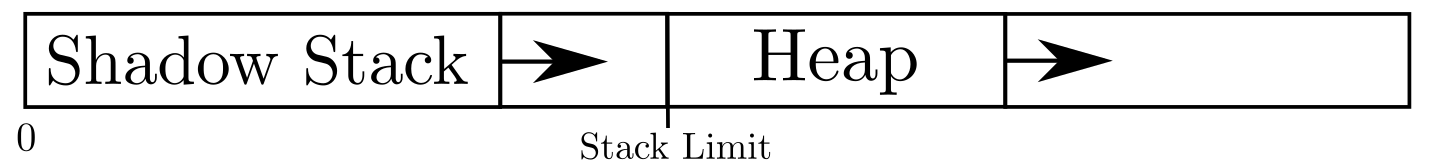
\includegraphics[scale=0.5]{gc_heap}
\caption{WebAssembly memory layout with a shadow stack}
\label{fig:wasm-shadow}
\end{figure}

% INCLUDE DIAGRAM OF HOW SHADOW STACKS WORK



%%%%%%%%%%%% ALL WRITTEN IN PRESENT TENSE FROM HERE ON, DOESN'T REALLY MAKE SENSE IN PAST TENSE? %%%

\section{Requirements analysis}
For this project to be successful, my compiler had to be able to compile OCaml programs that used just the integer, boolean, comparison and list standard library operations, and did not use the module or object layers of the language, or exceptions. This defined the minimum subset of OCaml being supported. Achieving this required implementing multiple translation passes, first from the OCaml compiler's front-end output to my intermediate representation, and then from that to WebAssembly. I planned to verify the correctness of the translation passes by a set of test OCaml programs using the language features being supported. To be able to execute the resulting WebAssembly, I also needed to build a runtime system, to provide operations such as memory allocation. 

I had to collect data measuring the performance of the code output by my compiler, comparing it against the three alternatives mentioned previously. Performance would be measured in terms of execution time, heap usage, and the size of the compiled code. This required writing a set of benchmark OCaml programs, with equivalent programs in C and Grain, and these benchmarks should have reflected a range of programming styles. Testing scripts were also necessary to compile each of these benchmarks, for each alternative, and collect data for the three metrics identified. The aim was to demonstrate an improvement compared to the alternatives, particularly Js\_of\_ocaml, due to the inefficiencies of compiling OCaml to JavaScript mentioned in the introduction.


%allowing it to be compared with alternative methods for running code on the web.  Hopefully, this will demonstrate an advantage compared to Js\_of\_ocaml, since WebAssembly is a strongly typed binary format, so is expected to execute faster than the equivalent JavaScript when compiling a strongly typed language, such as OCaml.

Implementing optimisations in the compiler was chosen as an extension, to help achieve this improvement. This required a set of analysis and optimisation passes on both the intermediate representation and WebAssembly stages of the compiler. I also aimed to extend the range of OCaml programs supported by my compiler, as floating-point and reference operations increase the range of benchmarks that could be considered. %, and would make writing them easier. 

Another extension was to implement a garbage collector, using a shadow stack to make local variables accessible during garbage collection. This would allow more memory intensive benchmarks to be considered and make the comparison of my compiler against the alternatives more realistic, by not ignoring the overhead of memory management. %, which is not a part of my core requirements due to the challenges anticipated with garbage collection in WebAssembly.



\section{Software engineering methodology}

% Repetitive - just the same as the requirements analysis
The project can be separated into several stages that had to be completed in sequence, following the stages of a typical compiler pipeline and outlined in the requirements analysis. Translation from the IR to WebAssembly was done in two smaller steps, and the runtime system was designed in parallel with the back-end of the compiler. Optimisations were only added once I had a working compiler, and could each be implemented independently. Since I used the OCaml compiler's front-end, my compiler was also written in OCaml, which helped improve my familiarity with the language features being implemented. Similarly, the runtime system was written in WebAssembly, except for the garbage collector, written in JavaScript due to its complexity and to allow modifying it more quickly. WebAssembly was the natural choice for interacting with programs compiled as WebAssembly, and again helped improve my understanding of the language.

This structure of mostly independent translation/optimisation passes lends itself to the Kanban methodology \cite{kanban}, which is an incremental approach to software development I have used before on team projects. Work was broken down into manageable tickets, most of which could be completed in a couple of days, building on the project incrementally. I used the Jira project-tracking platform from Atlassian to maintain a board of tickets \cite{jira}. Having a list of tasks in progress or blocked by other components, updated regularly, meant that elements of the project were not forgotten about and I could track how long each task was taking, identifying when a task was more complex than anticipated and needed to be further subdivided. The tickets were also a means of grouping ideas or issues with the pieces of work they affected, and I added more precise tickets to the backlog as the project progressed and it became clearer which elements to implement next.

%\subsection{Backups}

Both the project and dissertation were version-controlled using Git, backed up to GitHub daily and continually synced with OneDrive. %Commits were given meaningful commit messages, including the identifier of the ticket they were associated with, making it easier to navigate back to past changes if necessary. 
At the start of the project, I also checked that I could run the tools required, such as the OCaml and Grain compilers, on the MCS machines as a backup. 

%%%%%%%%%%%%%%%%%%%%%%%%%%%%%%%%%%%%%%%%%%%%%%%%%%%%%%%%%%

%The implementation of the compiler can be cleanly separated into building a minimal working compiler, and adding optimisations on top of that. The first of these lends itself to an incremental development strategy, as a compiler can be split into several key stages where the interface from one stage to the next significantly affects the complexity of the next stage. A compiler is typically divided into a front-end for parsing and type-checking, a middle-end for translation to a suitable intermediate representation and performing optimisations, and a back-end for generating WebAssembly code. I ultimately determined that my compiler should have two separate IRs, and so worked through these stages one at a time, starting from the typed output of the OCaml compiler front-end. 

% Also added language features this way
%After achieving a working compiler, iterative design becomes far more practical since I cannot accurately predict the benefit of different optimisations without repeated data collection on a range of benchmarks. For both stages of development, I decided to use a Kanban board to keep track of tasks. % By associating segments of work to numbered tickets, it would be easier to find specific changes once far into the project. 
%By keeping a backlog of tickets, this was an easy way to track extra features that needed implementing as I developed the compiler, and to keep ideas and issues grouped by the piece of work they affected. It also meant that I could see how long I had been working on each ticket, which was useful for identifying the tasks I needed to dedicate more time to or subdivide into more manageable tasks.

%\subsection{Tooling}

\subsection{Testing}
% Primarily test-driven development with Ocaml unit test samples for each feature. Sort of an integration test
% TODO: Specific unit tests for mock IR programs to check specific components e.g. free vars, number of locals needed
% More specific tests to check that optimisations handle complex cases correctly.
Language features were added to the compiler following test-driven development. Before adding a new primitive, language construct or optimisation, OCaml programs would be written using that feature, and the output of the OCaml interpreter on those files would be recorded. 
I wrote a script to compile and run each of these programs with my compiler, comparing their output with the expected values. This ensured that each new feature was implemented correctly, and that a change or new optimisation did not break any of the previous tests. % Additional tests were also added as I considered edge cases while implementing features, ensuring that they were not overlooked by future modifications.
Additionally, for tests added to verify that optimisations were performed safely, inspecting the output WebAssembly ensured that optimisations were being performed in the correct places. 

% The same process was helpful for ensuring optimisations were only performed where safe to do so, adding cases where incorrectly applying a transformation would break the program. This was most often where expressions in the program had side-effects that must be preserved, preventing some optimisations being applied.

%Optimisations were similarly tested against all prior test programs, and additional tests were added for where these optimisations were more likely to make a mistake. % More detail in implementation section?

Unit tests were written with OUnit \cite{ounit} for several of the utility functions involved in translation and optimisation. For example, checking that the free variables in IR programs  were computed correctly, or that removing an instruction from the flowgraph representation of a WebAssembly program correctly preserved the edges linking that node's successors and predecessors.


Testing whole translation passes was challenging, since translation often introduces several inefficiencies whilst still being correct, and the translation cannot be verified without running the full compiler pipeline and executing the output. Therefore, until the core stages of the compiler and runtime were built, I relied on pretty-printing code to display the intermediate representations for some sample programs. This allowed identifying any obvious errors by inspection, and was only relied on at the start of the project, before even a minimal pipeline had been written.
 %. Although this was unlikely to detect subtle errors, it was only relied on at the start of the project, when even a minimal pipeline did not yet exist.


% Should go at the top as this was the first form of testing?
% TODO: Is this worth mentioning? Probably the first thing I want to cut out
%Testing individual stages of translation was challenging, since the intermediate representation produced would generally have several inefficiencies that later optimisation passes would remove, so could not be directly compared against some expected output. Similarly, trying to write an interpreter for the IR output would be time consuming and error prone. As such, I checked the initial stages of my compiler were behaving as expected by adding pretty-printing code for the intermediate representations, and manually inspecting the output for a few simple test programs. This would highlight any significant errors, and was only necessary until a minimal compiler pipeline down to WebAssembly was implemented, making testing much easier.

%Unit tests were still written with OUnit \cite{ounit} for specific functions involved in translation, which could be verified in isolation. For example, manually building the IR or WebAssembly representation of a program, and verifying properties such as which variables are free in a function body, or which variables are live at each point in the body. The distinction here is that, while there is flexibility in the code produced to perform the operations described by a previous representation, the analyses used during translation have a precise meaning that can be verified. 

%Testing individual translation stages was challenging since I did not want to spend a large amount of time writing an interpreter for my IR, which would itself be prone to errors in handling the semantics of the IR, and checking the exact output of the translation would be impractical as the unoptimised compiler would introduce several unnecessary assignments and checks. Therefore, I initially checked these stages by adding pretty-printing code for the IR and manually inspecting the output for some of the test programs. The simplifications made by each IR made translated programs relatively easy to follow, and this was only necessary until the minimum compiler pipeline was implemented, then programs could be run as WebAssembly and be tested much easier. \\
% TODO: ACTUALLY DO THIS!
%I still wrote unit tests for the more complex utility functions involved in translation, which could be more easily verified. This included tests for identifying the free variables of a block of code (important for constructing closures) and for the number of separate values allocated at once (important for determining the number of local variables a function requires). This should be inflexible values so are not affected by the compiler initially being inefficient, hence later optimisations would not invalidate these tests.


\subsection{Tools used} % REFERENCES TO EVERYTHING
I worked on the project on my Windows laptop, using Windows Subsystem for Linux to run OCaml. Opam, the OCaml package manager, was used to manage the 
OCaml compiler and packages needed for the project. I used the OUnit package for writing unit tests, the Wasm package for some of the back-end functionality, such as %a data structure representing WebAssembly modules and 
utility functions to output WebAssembly to a binary file, and the Js\_of\_ocaml package as an alternative to my compiler. The project used the front-end of version 4.11.1 of the OCaml compiler, which was the latest version at the start of the project, although version 4.12.0 has since been released. 

% Unnecessary to mention Grain/Clang? Already brought up a few times as alternatives

I used the WebAssembly Binary Toolkit to translate between the binary and text format, both for producing a binary of the runtime system, and to inspect the output of my compiler on test programs. Node.js was used to run the output WebAssembly and perform benchmarking, and the project was developed using the IntelliJ IDE, available under its educational license.


\section{Legality}
I used of the front-end of the official OCaml compiler \cite{ocaml}, which is distributed under the GNU Lesser General Public License. My use of the compiler and modifications to it are therefore permitted, provided that I retain the original license in my project and highlight where modifications have been made. 

Benchmark programs were adapted from two existing sources \cite{chris00, benchmark-game}, one of which is also distributed under the GNU LGPL, and the other under the BSD-3 license. Therefore, modification is once again permitted, provided the original licenses are retained.



